\documentclass{standalone}
\usepackage{ tikz }
\usepackage{ xparse }
\input{macros/all}

\begin{document}
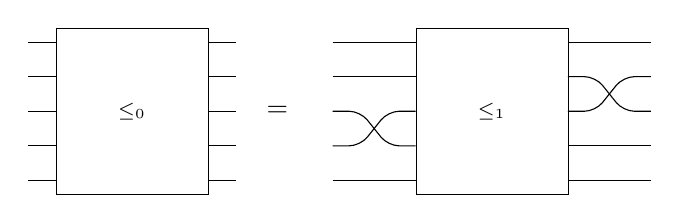
\begin{tikzpicture}[yscale=-1,x=1em,y=1.25em]
    \draw [rounded corners] (0,0) -- (1,0);
    \draw [rounded corners] (0,1) -- (1,1);
    \draw [rounded corners] (0,2) -- (1,2);
    \draw [rounded corners] (0,3) -- (1,3);
    \draw [rounded corners] (0,4) -- (1,4);

    \node[draw, minimum height = 6em, minimum width = 5.5em, anchor = west] at (1, 2){$\shuffle_{\leq_0}$};

    \draw [rounded corners] (6.5,0) -- (7.5,0);
    \draw [rounded corners] (6.5,1) -- (7.5,1);
    \draw [rounded corners] (6.5,2) -- (7.5,2);
    \draw [rounded corners] (6.5,3) -- (7.5,3);
    \draw [rounded corners] (6.5,4) -- (7.5,4);

    \node at (9,2){$=$};

    \draw [rounded corners] (11,0) -- (14,0);
    \draw [rounded corners] (11,1) -- (14,1);
    \draw [rounded corners] (11,2) -- (12,2) -- (13,3) -- (14,3);
    \draw [rounded corners] (11,3) -- (12,3) -- (13,2) -- (14,2);
    \draw [rounded corners] (11,4) -- (14,4);

    \node[draw, minimum height = 6em, minimum width = 5.5em, anchor = west] at (14, 2){$\shuffle_{\leq_1}$};

    \draw [rounded corners] (19.5,0) -- (22.5,0);
    \draw [rounded corners] (19.5,1) -- (20.5,1) -- (21.5,2) -- (22.5,2);
    \draw [rounded corners] (19.5,2) -- (20.5,2) -- (21.5,1) -- (22.5,1);
    \draw [rounded corners] (19.5,3) -- (20.5,3) -- (21.5,3) -- (22.5,3);
    \draw [rounded corners] (19.5,4) -- (20.5,4) -- (21.5,4) -- (22.5,4);

\end{tikzpicture}
\end{document}